%% Document created 05 March 2021 automatically 
%% from /Users/massimosotgia/Desktop/uni_at_DIFI/Lab_C03/setup.py 

%% Copyright (C) Mattia Sotgia et al. 2021
%% Using class lab_unige.cls
%                                                            
%                                                            
%   **                 **             ******   ****   ****   
%  /**                /**            **////** *///** */// *  
%  /**        ******  /**           **    // /*  */*/    /*  
%  /**       ´´´´´´** /******      /**       /* * /*   ***   
%  /**        ******* /**///**     /**       /**  /*  /// *  
%  /**       **´´´´** /**  /** **  //**    **/*   /* *   /*  
%  /********//********/****** /**   //****** / **** / ****   
%  ////////  //////// /////   //     //////   ////   /´///   
%                                                            
%                                                            
\documentclass[italian, a4paper, 10pt, twocolumn]{../../style/lab_unige}
\usepackage[a4paper, margin=1.25cm, footskip=0.25in]{geometry}

\usepackage[utf8]{inputenc}
\usepackage[T1]{fontenc}

\usepackage[italian]{babel}

% \usepackage{biblatex}

\usepackage[bookmarksopen=true, 
citebordercolor={0 1 0}, 
linkbordercolor={1 0 0}, 
urlbordercolor={0 1 1}]{hyperref}
\usepackage[numbered]{bookmark}

\usepackage{graphicx}
\graphicspath{{../fig/}}
\usepackage{array}
\usepackage{tabulary}
\usepackage{booktabs}

% FOUNDAMENTAL
\usepackage{../../style/custom}

\usepackage{physics}

\usepackage{breqn}
\usepackage{cuted}
\usepackage{txfonts}

\usepackage{lipsum}

%% Define ref types
\newcommand{\reftab}[1]{Tab. {\ref{#1}}}%
\newcommand{\reffig}[1]{Fig. {\ref{#1}}}%
\newcommand{\refeqn}[1]{({\ref{#1}})}%
%% PAPER ONLY custom Macros
\newcommand{\gLab}{$g_t=(9.8056\pm0.0001 \text{ stat}) \text{ m/s}^2$\space}
\newcommand{\ks}{$k_{\text{\small statico}}$\space}
\newcommand{\kd}{$k_{\text{\small dinamico}}$\space}
\newcommand{\ChiSqr}{$\chi^2$\space}
\newcommand{\ChiNdf}{$\chi^2/\text{ndf}$\space}
\newcommand{\cernroot}{\texttt{root} \space}
\newcommand{\scidavis}{\texttt{scidavis} \space}
\newcommand{\treSigma}{$3\sigma$\space}
\newcommand{\stdNG}[2]{$S_{#1}$($#2$)} %<- ???
\newcommand{\stdErr}[1]{$\varepsilon_{#1}$}
\newcommand{\hookeLaw}{$F=k\cdot\delta l$\space}
\newcommand{\misuraIncertezaUM}[3]{$#1\pm#2$ #3}
\newcommand{\Lo}{$l_0$\space}
\newcommand{\Li}[1]{$l_{#1}$}
\newcommand{\Ti}[1]{$T_{#1}$}
\newcommand{\MassI}[1]{$m_{#1}$}


%%
\setlength{\columnsep}{6mm}

\begin{document}
    \twocolumn[
    \begin{@twocolumnfalse}
        \title{
            Verifica Sperimentale della Legge di Hooke con Metodo Statico e Dinamico
        }
        \author{
        Eugenio Dormicchi\textsuperscript{1},
        % Riccardo Pizzimbone\textsuperscript{1}, 
        Giovanni Oliveri\textsuperscript{1},
        Mattia Sotgia\textsuperscript{1, 2}
        }

        \date{
        \textsuperscript{1}Gruppo C03, Esperienza di laboratorio n. 5 \\
        \textsuperscript{2}In presenza in laboratorio per la presa dati\\
            % Università degli Studi di Genova, Dipartimento di Fisica.\\
            Presa dati-- 
            10 Marzo 2021, 15:00-- 18:00; Analisi dati-- 
            16 Marzo 2021
        }
        \maketitle
        
        \begin{abstract}
            \textit{Obiettivo--}
            Vogliamo verificare la validità della legge di Hooke per cui la forza $\va{F}$ applicata su un corpo 
            elastico è direttamente proporzionale all'elongazione causata, secondo la legge \hookeLaw.
            \textit{Metodi--}
            Sfruttiamo due modelli per ricavare in modo differente la costante $k$ legata alla molla. Considerando 
            la molla in una condizione statica, con un corpo di massa nota \MassI{i}, e misurando l'allungamento 
            \Li{i} causato dalla massa, possiamo ricavare \ks. Se invece mettiamo in oscillazione dalla condizione 
            di equilibrio \Lo possiamo dal periodo \Ti{i} ricavare \kd (considerando il moto nel regime elastico).
            \textit{Risultati--}
        
            \textit{Conclusione--}
        
        
        \end{abstract}
        \vspace{2em}
    \end{@twocolumnfalse}
    ]

    %%%% CORPO DEL TESTO
    %%%% CORPO DEL TESTO

    \section{Obiettivo}
    \label{section:aim}
    Obiettivo dell'esperienza è quello di verificare la validità della relazione $\va{F}=k\delta\va{l}$ (che 
    possiamo considerare nel nostro caso \hookeLaw , poiché consideriamo solo componenti lungo lo stesso asse) 
    per cui la forza $\va{F}$ esercitata su un corpo elastico è direttamente proporzionale all'allungamento 
    causato dalla stessa forza, a meno di una costante $k$.
    Per verificare la legge di Hooke esguiamo misure su due modelli, uno statico e uno dinamico, e confrontiamo 
    graficamente il risultato ottenuto. 
    
    Infine vogliamo ricavare il valore rispettivamente di \ks e di \kd~, ed
    esegure una verifica della compatibilità dei valori. Se tali valori risultano compatibili infine proviamo a 
    ricavare il valore della miglior stima, ottenuto con una media pesata sugli errori associati.

    \section{Strumentazione}
    \label{section:strument}
    Abbiamo a disposizione come strumentazione:\\
    un calibro ventesimale di portata 20~cm e sensibilità 0.05~mm;\\
    un cronometro di portata molto maggiore alle misure effettuate e sensibilità 0.01~s;\\
    una bilancia elettronica KERN~BCP-350/4, di portata 350~g, considerando come sensibilità la linearità dello 
    strumento 0.04~g (non rischiamo così di sottostimare l'errore);\\
    un foglio di carta millimetrata attacato con le pinze su un piano verticale posto sulla struttura che sostiene
    la molla, parallelo a quest'ultima;\\
    una squadra utilizzata per ridurre l'errore commesso di parallasse;\\
    una vite infinita con un gancio all'estremità e due bulloni, necessario per fissare le masse alla molla;\\
    una molla di costante elastica $k$;\\
    diverse masse cilindriche forate, considerate di densità omogenea;\\

    La struttura utilizzata prevede una guida fissata al muro dove a un estremo è vincolata tramite un braccetto 
    una molla, libera per l'altro estremo. Sulla guida è collocato un piano mobile con sopra applicato il foglio 
    di carta millimetrata con due pinze. Tale piano viene fermato con due viti sulla guida all'altezza tale da
    posizionare l'estremo libero della molla in cima al foglio millimetrato. In qusto modo ci assicuriamo che 
    l'aggiunta del peso all'estremo della molla e la relativa elongazione rimangano nei limiti del foglio.

    \begin{figure}
        \centering
        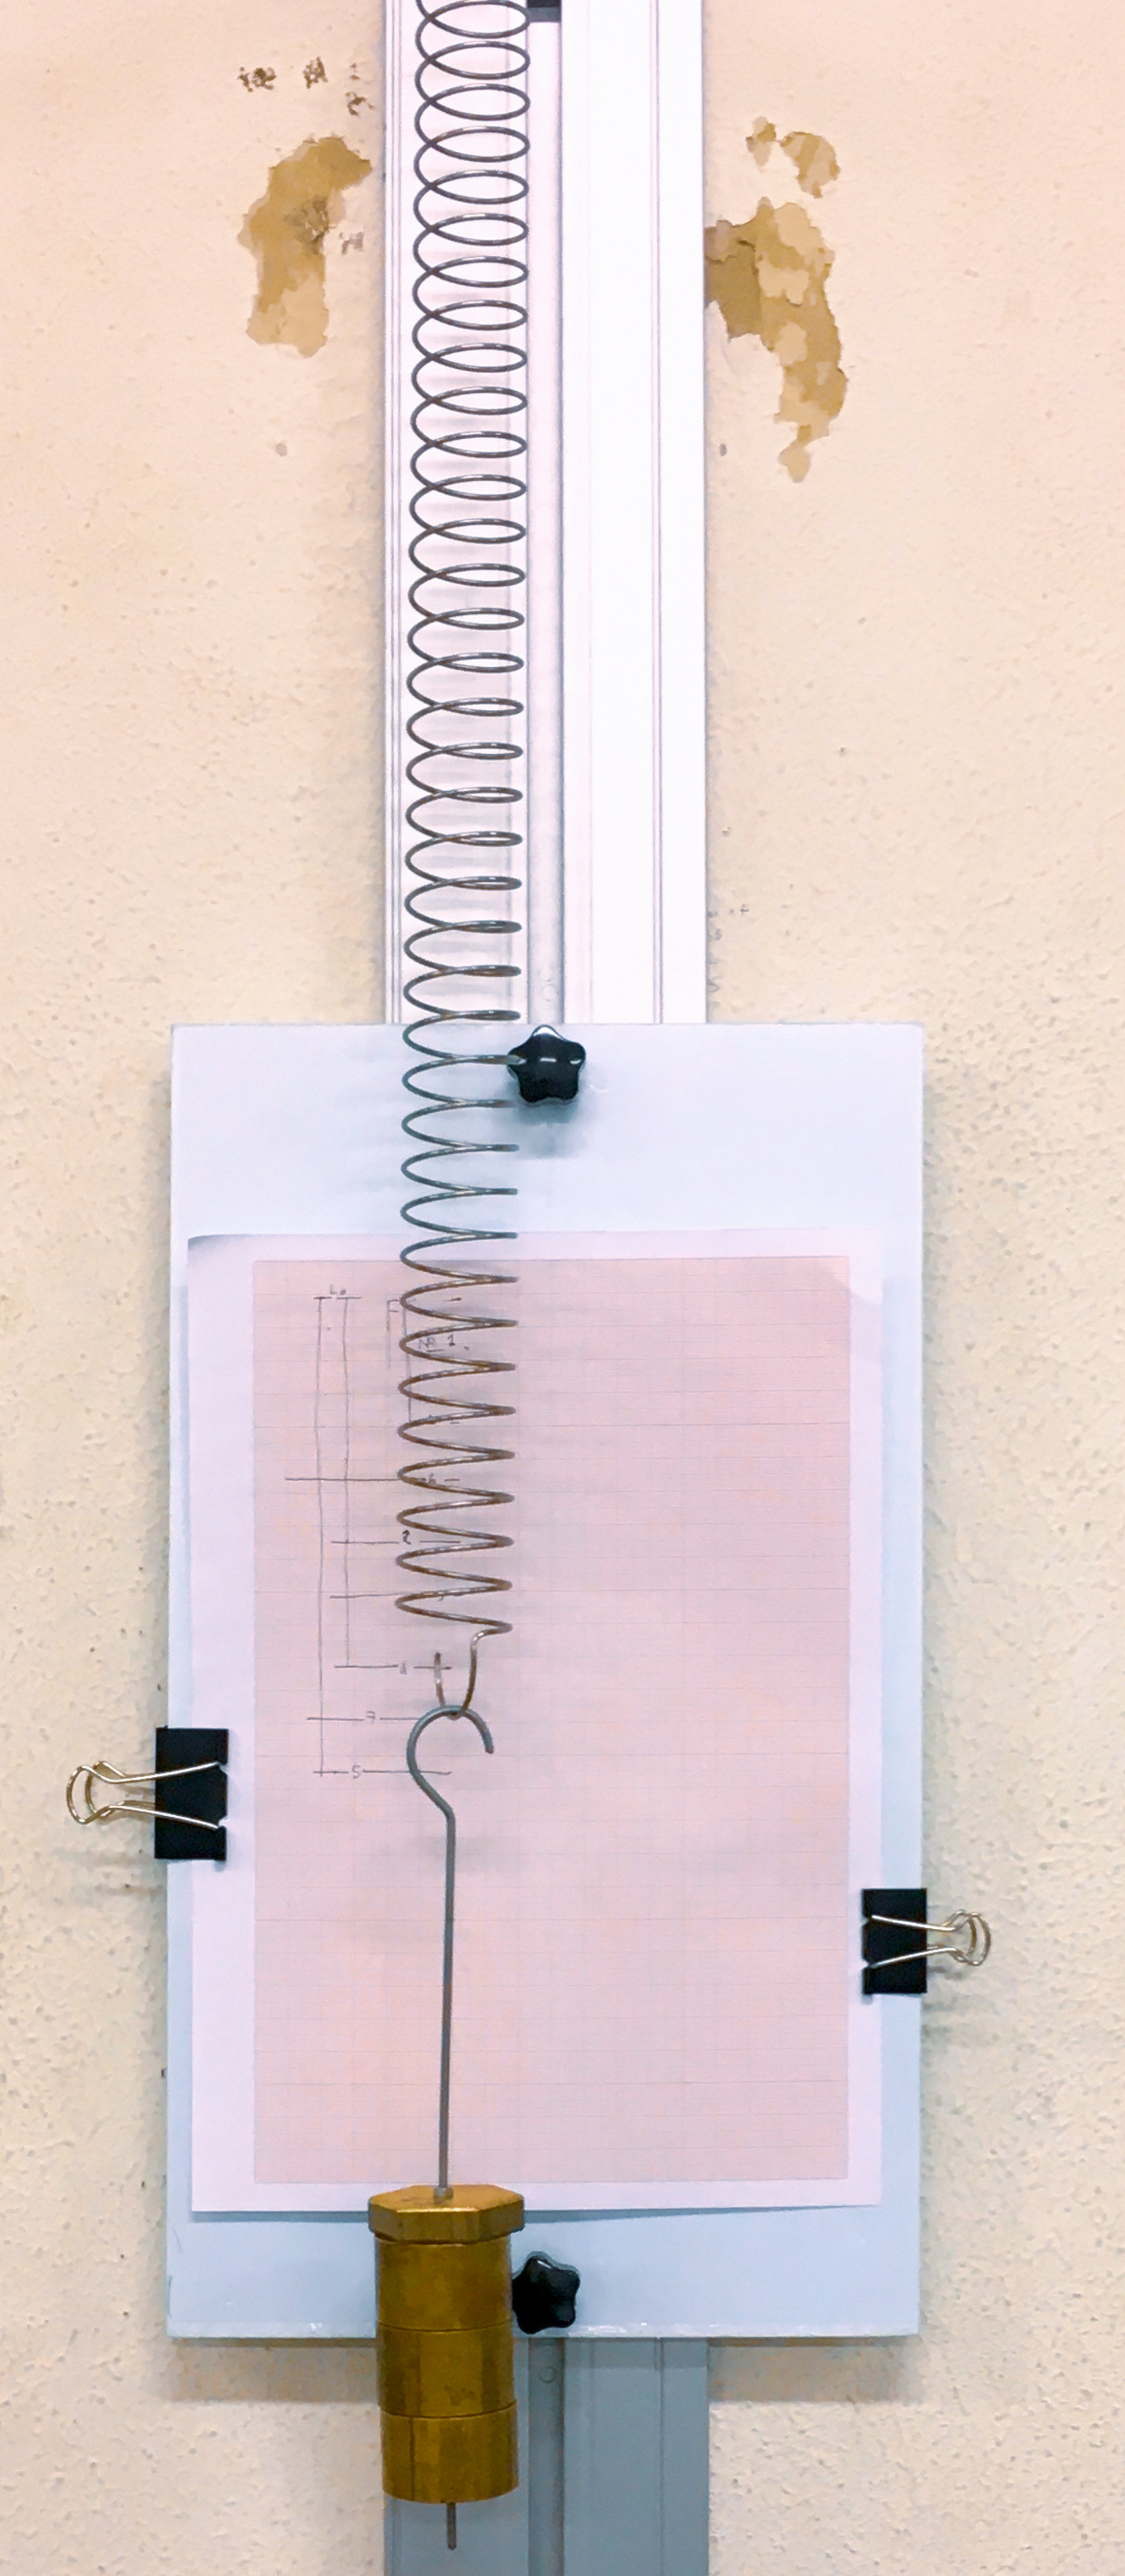
\includegraphics[width=0.8\linewidth]{IMG_0242.JPG}
        \caption{Apparato sperimentale}
        \label{figure:apparatus}
    \end{figure}

    \begin{figure*}[t]
        \centering
        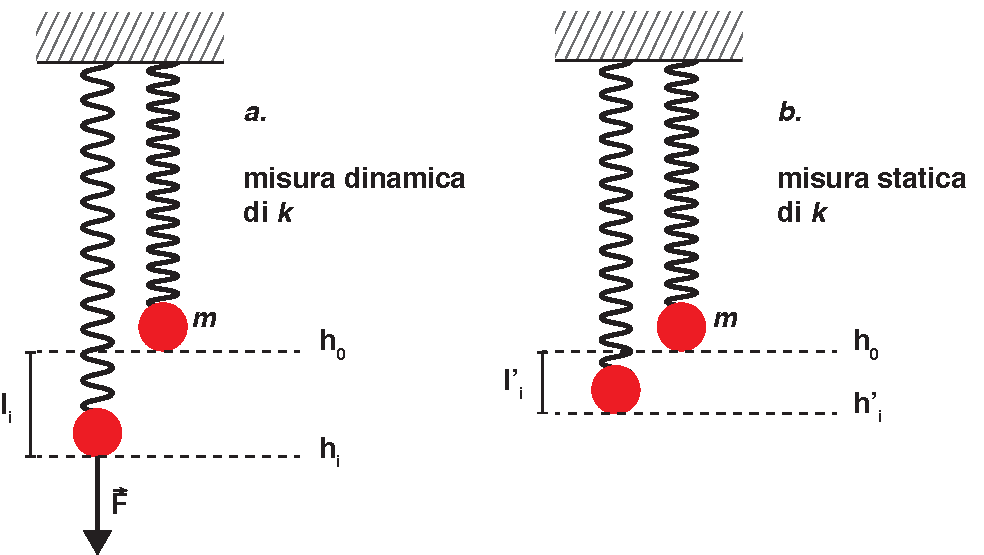
\includegraphics[width=0.8\linewidth]{system_horiz.pdf}
        \label{figure:methods}
        \caption{\textit{a.} \textit{b.}}
    \end{figure*}

    \section{Metodi}
    \label{section:methods}
    Tutte le misure sono riportate nelle unità del Sistema Internazionale (SI). Si assume come nota e costante 
    l'accelerazione di gravità \gLab .

    
    Si fa spesso riferimento anche alla regola del \treSigma, con la quale si vuole intendere la volontà di 
    trasformare un errore di tipo massimo in errore statistico, e quindi considerando il valore vero con una
    probabilità statistica del \treSigma~$\approx99.73\%$ di probabilità del dato vero.\\
    %% MAGARI AGGIUNGERE COMMENTO SU QUANTE CIFRE SI CONSIDERANO E COME APPROSSIMIAMO I VALORI %%
    I valori riportati sono stati approssimati tenendo conto di alcune convenzioni prese. Si approssima 
    l'errore ad una cifra significativa se tale cifra è $\geqslant3$, altrimenti se tale cifra è 1 o 2 allora
    si considerano due cifre significative. Considerando quindi le posizioni decimali significative dell'errore
    si approssima per eccesso il valore numerico della grandezza. 

    In entrambi i modelli la molla è sempre utilizzata in un regime elastico, tale per cui la molla è capace
    di ritornare alla condizione iniziale, e quindi in una condizione in cui l'energia totale del sistema si 
    conserva.

    Poichè la portata della bilancia elettronica è di 350~g e le masse da noi utlizzate combinate danno valori
    superiori, procediamo a pesare le masse in combinazioni tali da non superare tale limite della bilancia, 
    ma con lo scopo di non effettuare troppe misure sommate poichè l'errore totale della misua è la somma degli
    errori delle singole pesate. Inoltre per il medesimo motivo il gancio viene pesato in una delle pesate e 
    non singolarmente.

    Per riportare le misure di lunghezza raggiunte dalla molla sul foglio abbiamo utilizzato una squadra per 
    ridurre l'errore dovuto alla parallasse.\\

    Misuriamo la massa della molla utilizzando la squadra come piano d'appoggio per allargare il piatto della 
    bilancia. Tale massa risulta essere $83.894\pm0.004$~g.

    Segnamo sul foglio millimetrato la proiezione della lunghezza \Lo raggiunta dalla molla a riposo quando 
    essa è libera senza masse ulteriori appese. 

    \subsection{Metodo Statico}
    \label{subsec:methods_stat}
    Vogliamo ricavare tramite misure di statica un valore \ks (ovvero una misura di $k$).

    Dai pesetti componiamo una massa \MassI{i} tale che la massa rientri nel regime delle elongazioni elastiche 
    per la molla, ovvero che  $0.150 \text{ kg} < m_i < 1.200 \text{ kg}$. 
    Pesata quindi la massa totale (come somma delle diverse pesate) fissiamo sulla vite senza fine tramite i 
    bulloni i pesetti. Agganciamo dunque il sistema composto da masse + gancio alla molla, attendiamo che questa 
    si stabilizzi su una condizione di equlibrio e segniamo sul foglio la lunghezza raggiunta dall'estremo della 
    molla.
    Misuriamo dunque la variazione di elongazione $\delta l_i$, a cui associamo un errore di $\Delta l_i=$1~mm, 
    considerando come incertezza sulla misura il minimo valore misurabile dalla carta millimetrata. Convertiamo 
    poi l'errore assoluto in errore standard $\varepsilon_{l_i} = \Delta l_i /\sqrt{3}$ secondo la regola del 
    \treSigma.
    
    Ripetiamo questo procedimento per 7 misure di massa differenti, e trasciviamo i valori in tabella. %% <<-------INDICARE TABELLA!!!!!

    \subsection{Metodo dinamico}
    \label{subsec:methods_dyn}
    Per ogni massa utilizzata nel metodo statico effettuiamo anche una considerazione di tipo dinamico del 
    sistema, per ricavare un valore \kd da confrontare poi con \ks, per verificarne il valore.
    Applichiamo una forza $\va{F}$ al sistema molla + \MassI{i}, spostando la molla dalla sua posizione di 
    equilibrio di un $\delta x$ abbastanza piccolo. Questa necessità può essere spiegata da due fatti: 
    innanzitutto il periodo di oscillazione della sistema non dipende dall'ampiezza dell'oscillazione, e 
    inoltre un ampiezza maggiore porta ad avere una velocità maggiore e quindi, poichè l'attrito viscoso 
    dell'aria è direttamente proporzionale alla velocità $v$ ($\va{f_v}=-\beta \va{v}$) causando quindi 
    uno smorzamento del moto.\\
    Per dimostrare il primo punto, partendo dalle equazioni delle forse in gioco ricaviamo:
    \[
        \va{f_{el}} + \va{P} = M_{\text{tot}}\va{a}
    \]
    da cui 
    \[
        k\cdot x - M\cdot g = - M \cdot \ddot{x}
    \]
    Dividendo per la massa M
    \[
        \frac{k}{M}\cdot x - g = - \ddot{x}
    \]
    Se riscriviamo il termine $\frac{k}{M} \cdot (x - g\cdot\frac{M}{k}) = \xi$, osserviamo che 
    $\ddot{\xi} = \ddot{x}$, quindi possiamo riscrivere come
    \[
        - \frac{k}{M} \cdot \xi = \ddot{\xi}
    \]
    Se consideriamo il fattore $\frac{k}{M}$ questo ha dimensioni s$^{-1}$, quindi possiamo riscrivere
    \[
        - \omega^2 \cdot \xi = \ddot{\xi}
    \]
    Che è una equazione differenziale al secondo ordine, che se risolta ci dà proprio l'equazione del moto 
    armonico oscillatorio, dove però il termine $g \cdot \frac{M}{k}$ rappresenta la posizione $x_{\text{eq}}$
    di equilibrio. Da $\omega = \sqrt{k/M}$ possiamo ricavare il periodo di oscillazione del sistema.\\
    Se infatti il periodo è $T = \frac{2 \pi}{\omega}$, allora otteniamo
    \[
        T = 2 \pi \sqrt{\frac{M}{k}}
    \]
    che denota la non dipendenza del periodo dall'ampiezza di oscillazione. 

    \section{Risultati}
    \label{section:results}

    % \begin{table}[t]
    \centering
    \small
    \caption{Valori delle masse e relativi valori di periodo $\bar{T_i}$. Sono riportati anche i valori di
    $\bar{T_i^2}$. Gli errori relativi ai periodi sono ricavati dal calcolo dell'errore standard ($\varepsilon$). 
    L'errore sulla massa preso dalla linearità dello strumento (0.004 g) è ottenuto dalla somma degli errori dovuti 
    alle diverse pesate. Il valore è poi staticizzato per la regola del \treSigma ($\varepsilon_m = \delta m/\sqrt{3}$)}
    \label{table:dyn_values}
    \begin{tabular}{lccc}
        \hline\hline\\[-1.5ex]
          & $m_i\pm\varepsilon_m$ & Periodo $\bar{T_i}\pm\varepsilon_T$ & Periodo al quadrato $\bar{T_i^2}\pm\varepsilon_{T^2}$ \\[+0.5ex] \hline \\[-1.5ex]
        1 & 0.261499$\pm$2e-06    & $0.3761\pm0.0015$                   & $0.1415\pm0.0011$                                     \\[+0.5ex]
        2 & 0.650447$\pm$7e-06    & $0.5646\pm0.0020$                   & $0.3188\pm0.0022$                                     \\[+0.5ex]
        3 & 0.796669$\pm$7e-06    & $0.6217\pm0.0018$                   & $0.3865\pm0.0022$                                     \\[+0.5ex]
        4 & 1.035634$\pm$9e-06    & $0.6962\pm0.0011$                   & $0.4847\pm0.0015$                                     \\[+0.5ex]
        5 & 0.393091$\pm$5e-06    & $0.439 \pm0.003 $                   & $0.1925\pm0.0027$                                     \\[+0.5ex]
        6 & 0.916857$\pm$9e-06    & $0.6574\pm0.0017$                   & $0.4322\pm0.0021$                                     \\[+0.5ex]
        \hline \\[-1.5ex]
        
    \end{tabular}
\end{table}

    \section{Conclusione}
    \label{section:conclusion}

    \subsection{Controlli}

    \subsection{Possibili errori sistematici}
    
    \appendix

    \section{Dati completi}
    %%includere tabelle dati completi periodi e calcolo periodi.

\end{document}
    
